\RequirePackage{luatex85}
\documentclass[tikz, border=10pt]{standalone}
\usetikzlibrary{shapes.geometric, arrows}
\usetikzlibrary{positioning}

\tikzstyle{selection} = [rectangle, rounded corners, minimum width=3cm, minimum height=1.2cm, text centered, text width=3.5cm, draw=black, fill=white]
\tikzstyle{hemisphere} = [rectangle, rounded corners, minimum width=2cm, minimum height=0.8cm, text centered, text width=3.5cm, fill=white]

\tikzstyle{arrow} = [thick,->,>=stealth]

\begin{document}

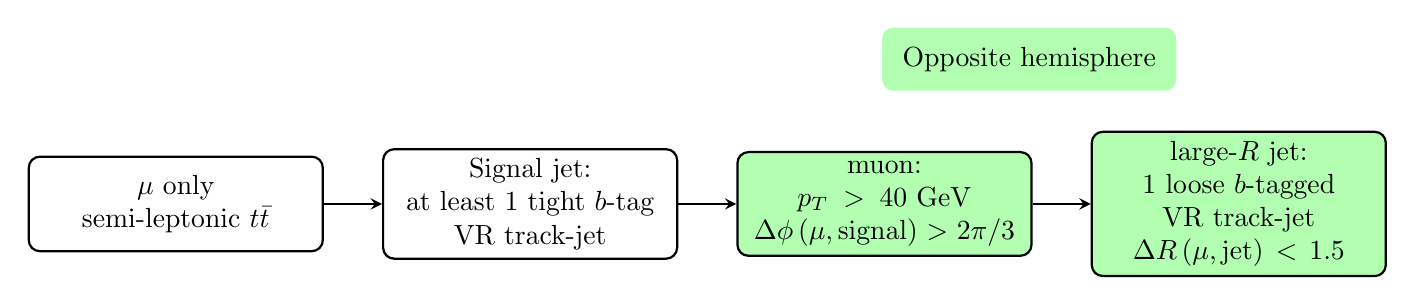
\begin{tikzpicture}[thick, node distance=2cm]
 \node (semi-leptonic) [selection] {$\mu$ only\\semi-leptonic $t\bar{t}$};
 \node (b-tag) [selection, right of=semi-leptonic, node distance=4.5cm] {Signal jet: \\at least 1 tight $b$-tag\\VR track-jet};
 \node (muon) [selection, right of=b-tag, node distance=4.5cm, fill=green!30] {muon:\\$p_{T} > 40~\mathrm{GeV}$ $\Delta\phi\left(\mu, \mathrm{signal}\right) > 2\pi/3$};
 \node (Wjets) [selection, right of=muon, node distance=4.5cm, fill=green!30] {large-$R$ jet:\\1 loose $b$-tagged VR track-jet\\$\Delta R\left(\mu, \mathrm{jet}\right) < 1.5$};
 \node (hemisphere) [hemisphere, above right of=muon, node distance=2.6cm, fill=green!30] {Opposite hemisphere};

 \draw [arrow] (semi-leptonic) -- (b-tag);
 \draw [arrow] (b-tag) -- (muon);
 \draw [arrow] (muon) -- (Wjets);
\end{tikzpicture}
\end{document}
